%%%%%%%%%%%%%%%%%%%%%%%%%%%%%%%%%%%%%%%%%%%%%%%%%%%%%%%%%%%
% Chapter 3
\chapter{RFQ Data Set} \label{Ch3:title}
\begin{singlespacing}
\begin{microabstract}
   This chapter presents the RFQ data time-series which was generated as part of this thesis for the predictability and hidden state inference investigation. It provides graphical descriptions of the data, along with justification for choosing a 'binning' methodology to process the time-series. Finally it presents the model training, validation and test split methodology used as well as the required transformations performed using data wrangling techniques.
\end{microabstract}
\end{singlespacing}


\section{Data generation and descriptive statistics}

The RFQ time-series data was generated for the purpose of this investigation based on EURUSD currency pair and product type European vanilla option. The frequency of RFQs is representative of typical patterns of activity observed centred on London trading hours. This resulted in 44,687 RFQs generated over a period of 1 month. Table~\ref{Ch6Tab:1} is a snapshot of the first 9 entries in the RFQ data set.

\begin{table}[!ht]\centering\footnotesize\setlength{\tabcolsep}{3pt}
    \caption{Ordered extract of generated RFQ data}\label{Ch6Tab:1}
    \resizebox{\linewidth}{!}{\begin{tabular}{*{10}{c}}
        \toprule
            \bfseries ID &
            \bfseries QUOTE\_TIME\_UTC &
            \bfseries CCY\_PAIR &
            \bfseries SIDE &
            \bfseries PRODUCT &
            \bfseries NOTIONAL &
            \bfseries CALL\_PUT &
            \bfseries STRIKE &
            \bfseries EXPIRY\_DATE &
            \bfseries PREMIUM\\
        \midrule
        %
        1 & 30/10/17 00:19 & EURUSD & Buy & European & 1,000,000  & C & 1.168  & 13/11/17 & 4,060   \\
        %
        2 & 30/10/17 00:56 & EURUSD & Buy & European & 1,000,000  & C & 1.174  & 13/11/17 & 2,380   \\
        %
        3 & 30/10/17 01:18 & EURUSD & Buy & European & 1,000,000  & C & 1.178  & 13/11/17 & 1,610   \\
        %
        4 & 30/10/17 01:57 & EURUSD & Buy & European & 20,000,000 & C & 1.17   & 14/12/17 & 187,800 \\
        %
        5 & 30/10/17 02:28 & EURUSD & Buy & European & 1,000,000  & C & 1.1697 & 03/11/17 & 1,870   \\
        %
        6 & 30/10/17 02:58 & EURUSD & Buy & European & 1,000,000  & C & 1.1607 & 06/11/17 & 5,350   \\
        %
        7 & 30/10/17 03:20 & EURUSD & Buy & European & 500,000    & P & 1.14   & 30/01/18 & 2,571   \\
        %
        8 & 30/10/17 03:55 & EURUSD & Buy & European & 500,000    & C & 1.18   & 30/01/18 & 4,589   \\
        %
        9 & 30/10/17 04:20 & EURUSD & Buy & European & 500,000    & C & 1.18   & 30/01/18 & 4,591   \\
        \bottomrule
    \end{tabular}}
\end{table}

This data set would typically form a subset of a SDP's RFQ data set, which would include at least G11 currencies as well as other option product types (American options, target forwards, Accumulators etc.). For simplicity the focus for this thesis was the RFQ subset generated.

\subsubsection{'Binning' methodology}

In order to prepare RFQ data for suitable analysis a decision had to be made upfront on how best to represent the RFQ time-series. The two approaches considered were `binning' and `time-intervals'. The binning approach involves bucketing discrete RFQs into `bins' of equal width (for example 15minute bins). The `time-interval' approach would measure the differences in time between subsequent times. It was decided that the `binning' approach would be more suited to predicting the probability of a RFQ in the next `bin' due to the high frequency of RFQs especially in peak activity times. Also, the prediction of time intervals was not a realistic real-life scenario given the proximity of the RFQs.

As such the RFQ data was bucketed into 15 minutes `bins', with each `bin' assigned the number of RFQs in that 15min slot. To demonstrate the distribution of RFQ binned data a histogram plot of the count frequency is presented in Figure~\ref{Ch3Fig:1}. The plot shows that the count distribution is dominated by `bins' with zero RFQ requests, this makes sense when you consider all the non-peak times in any given day when there are few requests. 

\begin{figure}[!ht]\centering
    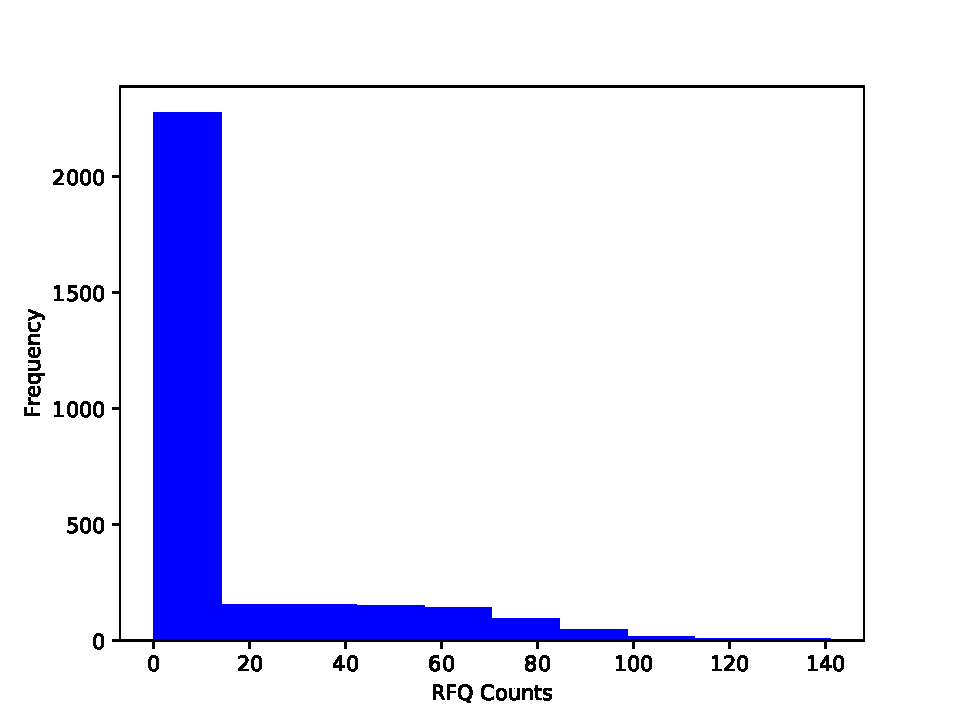
\includegraphics[width=0.8\linewidth]{./figures/Ch6fig1.pdf}
    \caption{Histogram plot of RFQ count frequency}\label{Ch3Fig:1}
\end{figure}

This appears to follow a power-law distribution below, where $x$ obeys a power law if drawn from a probability distribution where $\alpha$ is the scaling or exponent parameter and C is a normalisation constant \autocite{clauset2009power}.

\begin{equation}\label{Ch6Eq1}
    p(x) = C x^{-\alpha}
\end{equation}

Figure~\ref{Ch6Fig:2} presents a plots the best fit power law and the frequency counts data . Intervals where zero counts were observed was removed to fit the power law. The parameters for equation~\ref{Ch6Eq1} were found to be $C = 219.956$ and $\alpha = 0.826$.

\begin{figure}[!ht]\centering
    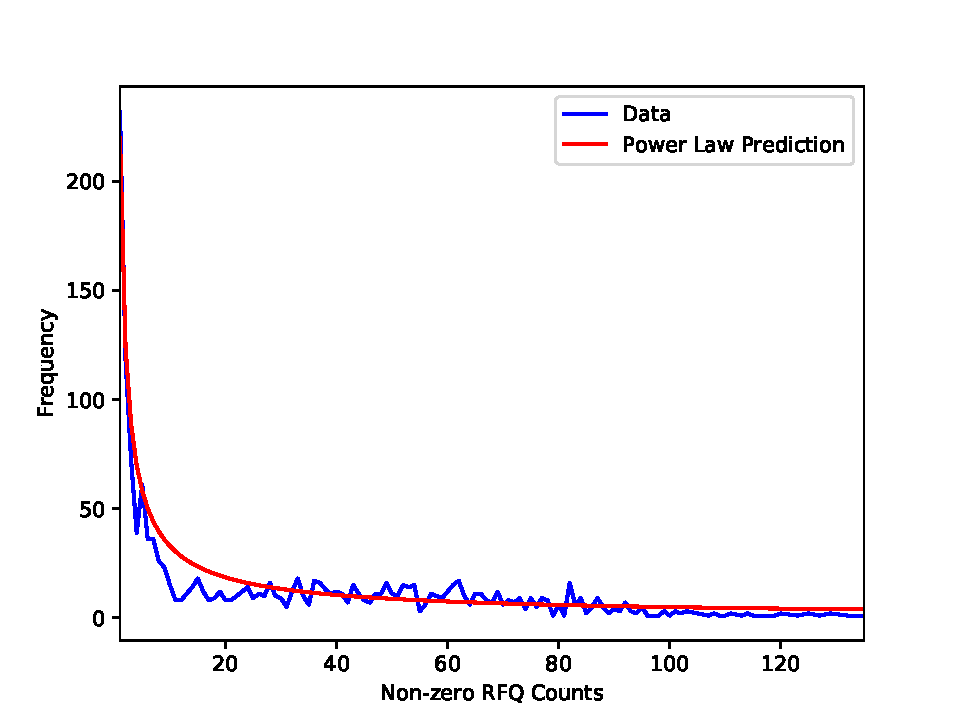
\includegraphics[width=0.8\linewidth]{./figures/Ch6fig2.pdf}
    \caption{Plot of best fit power law distribution}\label{Ch6Fig:2}
\end{figure}


Figure~\ref{Ch6Fig:2} shows the 44,687 RFQ data count distribution over the 1-month period. This clearly shows there is heightened RFQ activity daily with quitter periods in between peak times.

\begin{figure}[!ht]\centering
    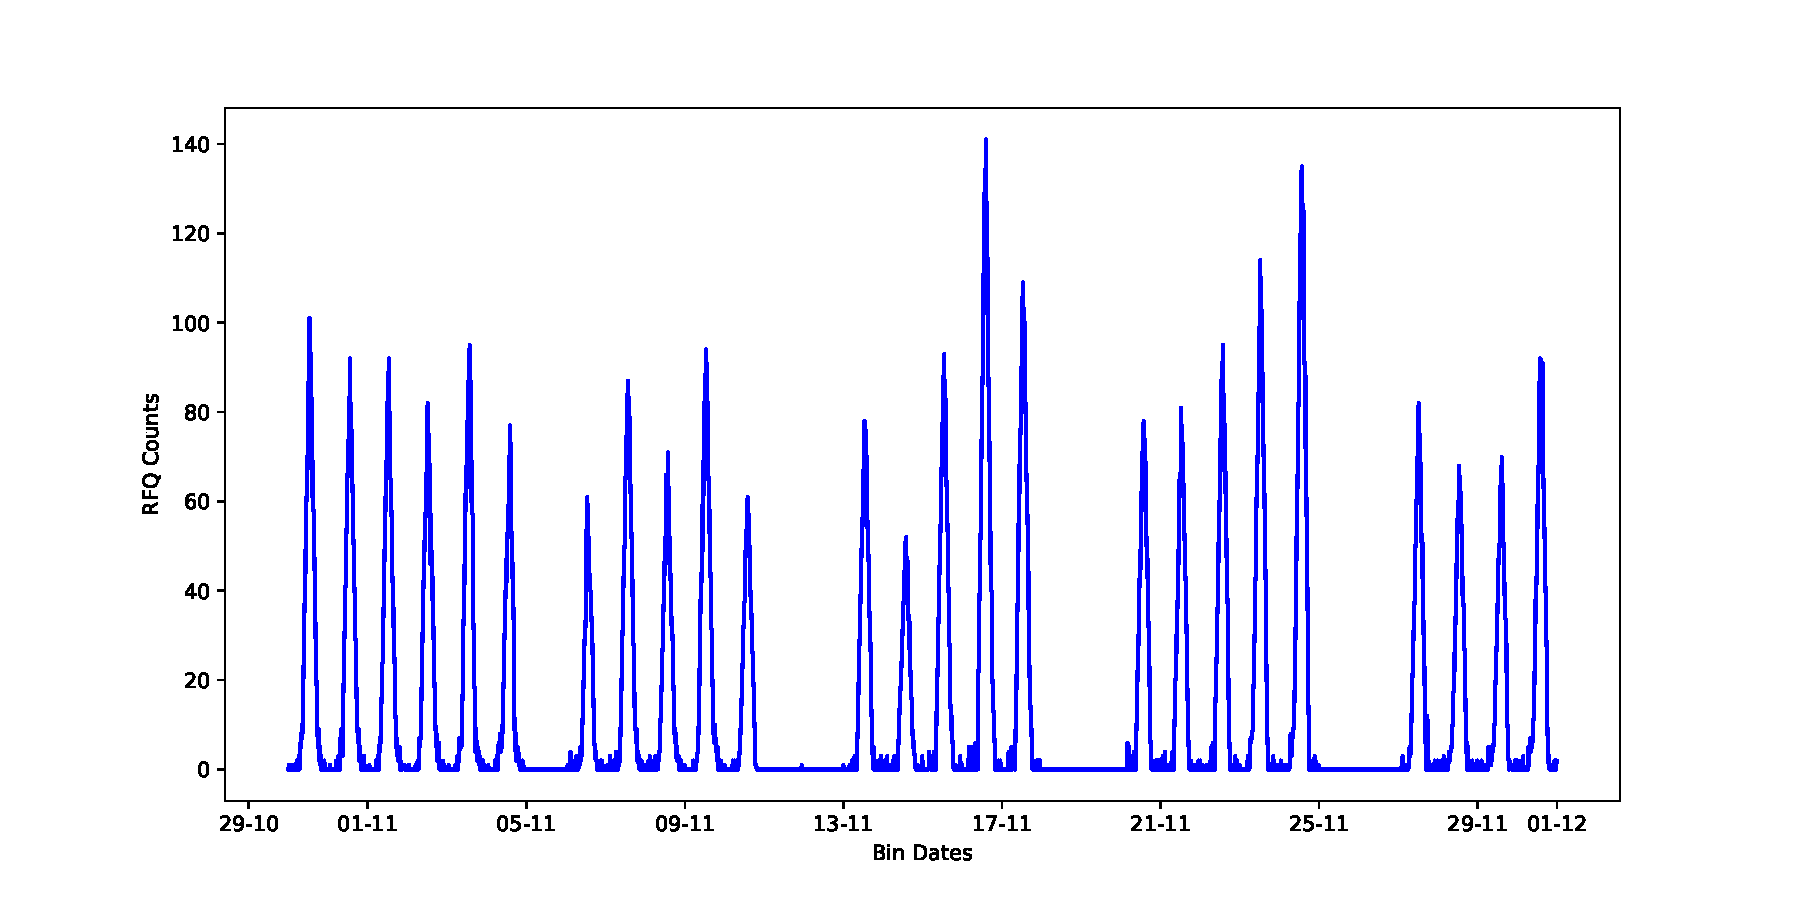
\includegraphics[width=0.8\linewidth]{./figures/Ch6fig3.pdf}
    \caption{Distribution of RFQ data over a period of 1 month}\label{Ch6Fig:3}
\end{figure}

The distribution for EURUSD RFQ for any given day broadly follows the pattern shown in Figure~\ref{Ch6Fig:4}. This is in line with the expectation of London trading hours. The RFQ activity starts to ramp up from 8am to around midday then starting to tail off until early evening when its level again with RFQs from other time zones. It is expected that there will be peaks around significant political or economic news.

\begin{figure}[!ht]\centering
    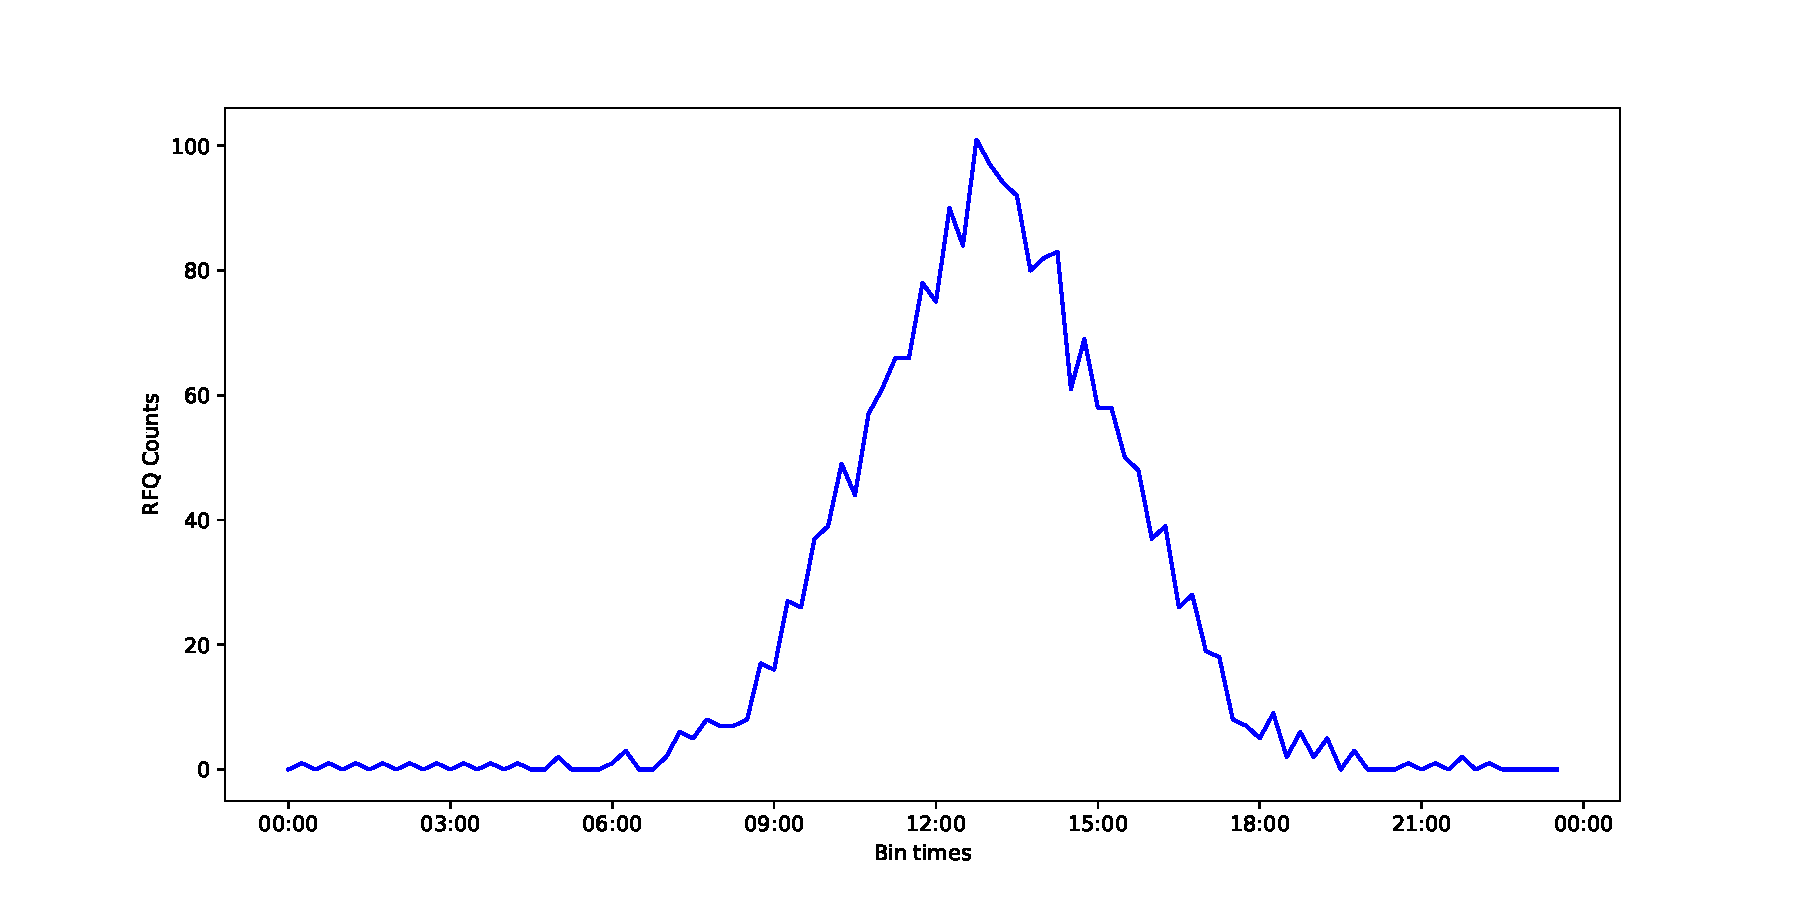
\includegraphics[width=0.8\linewidth]{./figures/Ch6fig4.pdf}
    \caption{Distribution of RFQ data over a single day}\label{Ch6Fig:4}
\end{figure}

\section{Data split and wrangling}\label{splitwrangle}
\subsection{Data train-test split}\label{train-testsplit}
The schematic in Figure~\ref{Ch7Fig:1} describes how the RFQ data is split for training, validation and testing. Broadly the steps apply to both our supervised and unsupervised models, which we are investigating however there are some differences with respect to the HMM model, which will be highlighted. The 4 stages highlighted in Figure~\ref{Ch7Fig:1} are explained further below:
\begin{enumerate}
    \item \textit{RFQ train-test split} -- this divides our data set into 2 subsets of training and test, which the model is first trained on and subsequently tested on to provide an unbiased evaluation of the performance. Note, the test data is set aside and untouched until the end to see how well the best model generalizes. The train portion of this split is used for cross-validation.
    \item \textit{Cross-Validation} -- the training portion of the dataset is used in this section. A k-fold cross-validation approach is taken using the either the default or a selected set of hyper-parameters to be tuned. The model is trained on k-1 folds as the training data and the resulting model then validated on the remaining part of the data (labelled validation) to establish performance measures such as Score or RMSE. The cross-validation then reports the average values computed overall and selects the best model.
    \item \textit{Re-Training} -- the model is then retrained on the training set using the best hyper-parameters and model performances are reported officially for the training set e.g. Score and RMSE.
    \item \textit{Testing} -- this is the final step to evaluate how well the trained model generalises to a real world scenario. Performance measures such as RMSE and Scores would be reported for the test data set.
\end{enumerate}

\begin{figure}[!ht]\centering
    \begin{tikzpicture}[x=20pt,y=20pt]
        \draw[dashed] (-2,0) -- (14,0);
        \foreach \x  in {-1.2,10,13} {\draw[dashdotted] (\x,-2) -- (\x,12);}
        \draw (-3.75,0) rectangle (-2.25,10);\node[rotate=90,font=\scriptsize] at (-3,5) {training \& validation};
        \fill[COL2,draw=black] (-3.75,0) rectangle (-2.25,-2);\node[rotate=90,font=\scriptsize] at (-3,-1) {test};
        \fill[COL2,draw=black] (13.75,0) rectangle (15.25,-2);\node[rotate=90,font=\scriptsize] at (14.5,-1) {test};
        \draw (10.75,0) rectangle (12.25,10);

        \begin{scope}[every node/.style={circle,draw,inner sep=1pt},font=\footnotesize]
            \node (N1) at (-3,11.5) {1};
            \node (N2) at ( 5,11.5) {2};
            \node (N3) at (11.5,11.5) {3};
            \node (N4) at (14.5,11.5) {4};
        \end{scope}
        \begin{scope}[every node/.style={below,minimum width=1cm,align=center,font=\scriptsize}]
            \node at (N1.south) {Data Split};
            \node at (N2.south) {Cross-validation};
            \node at (N3.south) {Re-train on\\ training set};
            \node at (N4.south) {Use same model\\ as (3) on\\ test data};
        \end{scope}

        \foreach \y in {0,...,4} {
            \foreach \x in {0,2,...,8} {
                \draw (\x,2*\y) coordinate (N\x\y) rectangle ++ (1,2);
            }
        }
        \foreach \x/\y in {0/4,2/3,4/2,6/1,8/0} {
            \fill[COL1,draw=black] (N\x\y) rectangle ++ (1,2);
            \draw [decorate,decoration={brace,amplitude=5pt}]
                ([shift={(-2pt,0pt)}]N\x\y) -- ++(0,2)
                node [black,midway,above,rotate=90,font=\scriptsize,yshift=3pt] {validation};
        }
            \draw [decorate,decoration={brace,amplitude=5pt}]
                ([shift={(-2pt,0pt)}]N00) -- ([shift={(-2pt,0pt)}]N04)
                node [black,midway,above,rotate=90,font=\scriptsize,yshift=3pt] {training};

            \draw [decorate,decoration={brace,amplitude=5pt}]
                ([shift={(0pt,-10pt)}]N80) -- ([shift={(0pt,-10pt)}]N00)
                node [black,midway,below,font=\scriptsize,yshift=-3pt] {Select hyperparameters};

            \draw [decorate,decoration={brace,amplitude=5pt}]
                (12.5,-10pt) -- (10.5,-10pt)
                node [black,midway,below,font=\scriptsize,yshift=-3pt,text width=2cm,align=center] {training using best hyper-parameters and recording performance metrics e.g. RMSE/MSE};
    \end{tikzpicture}
    %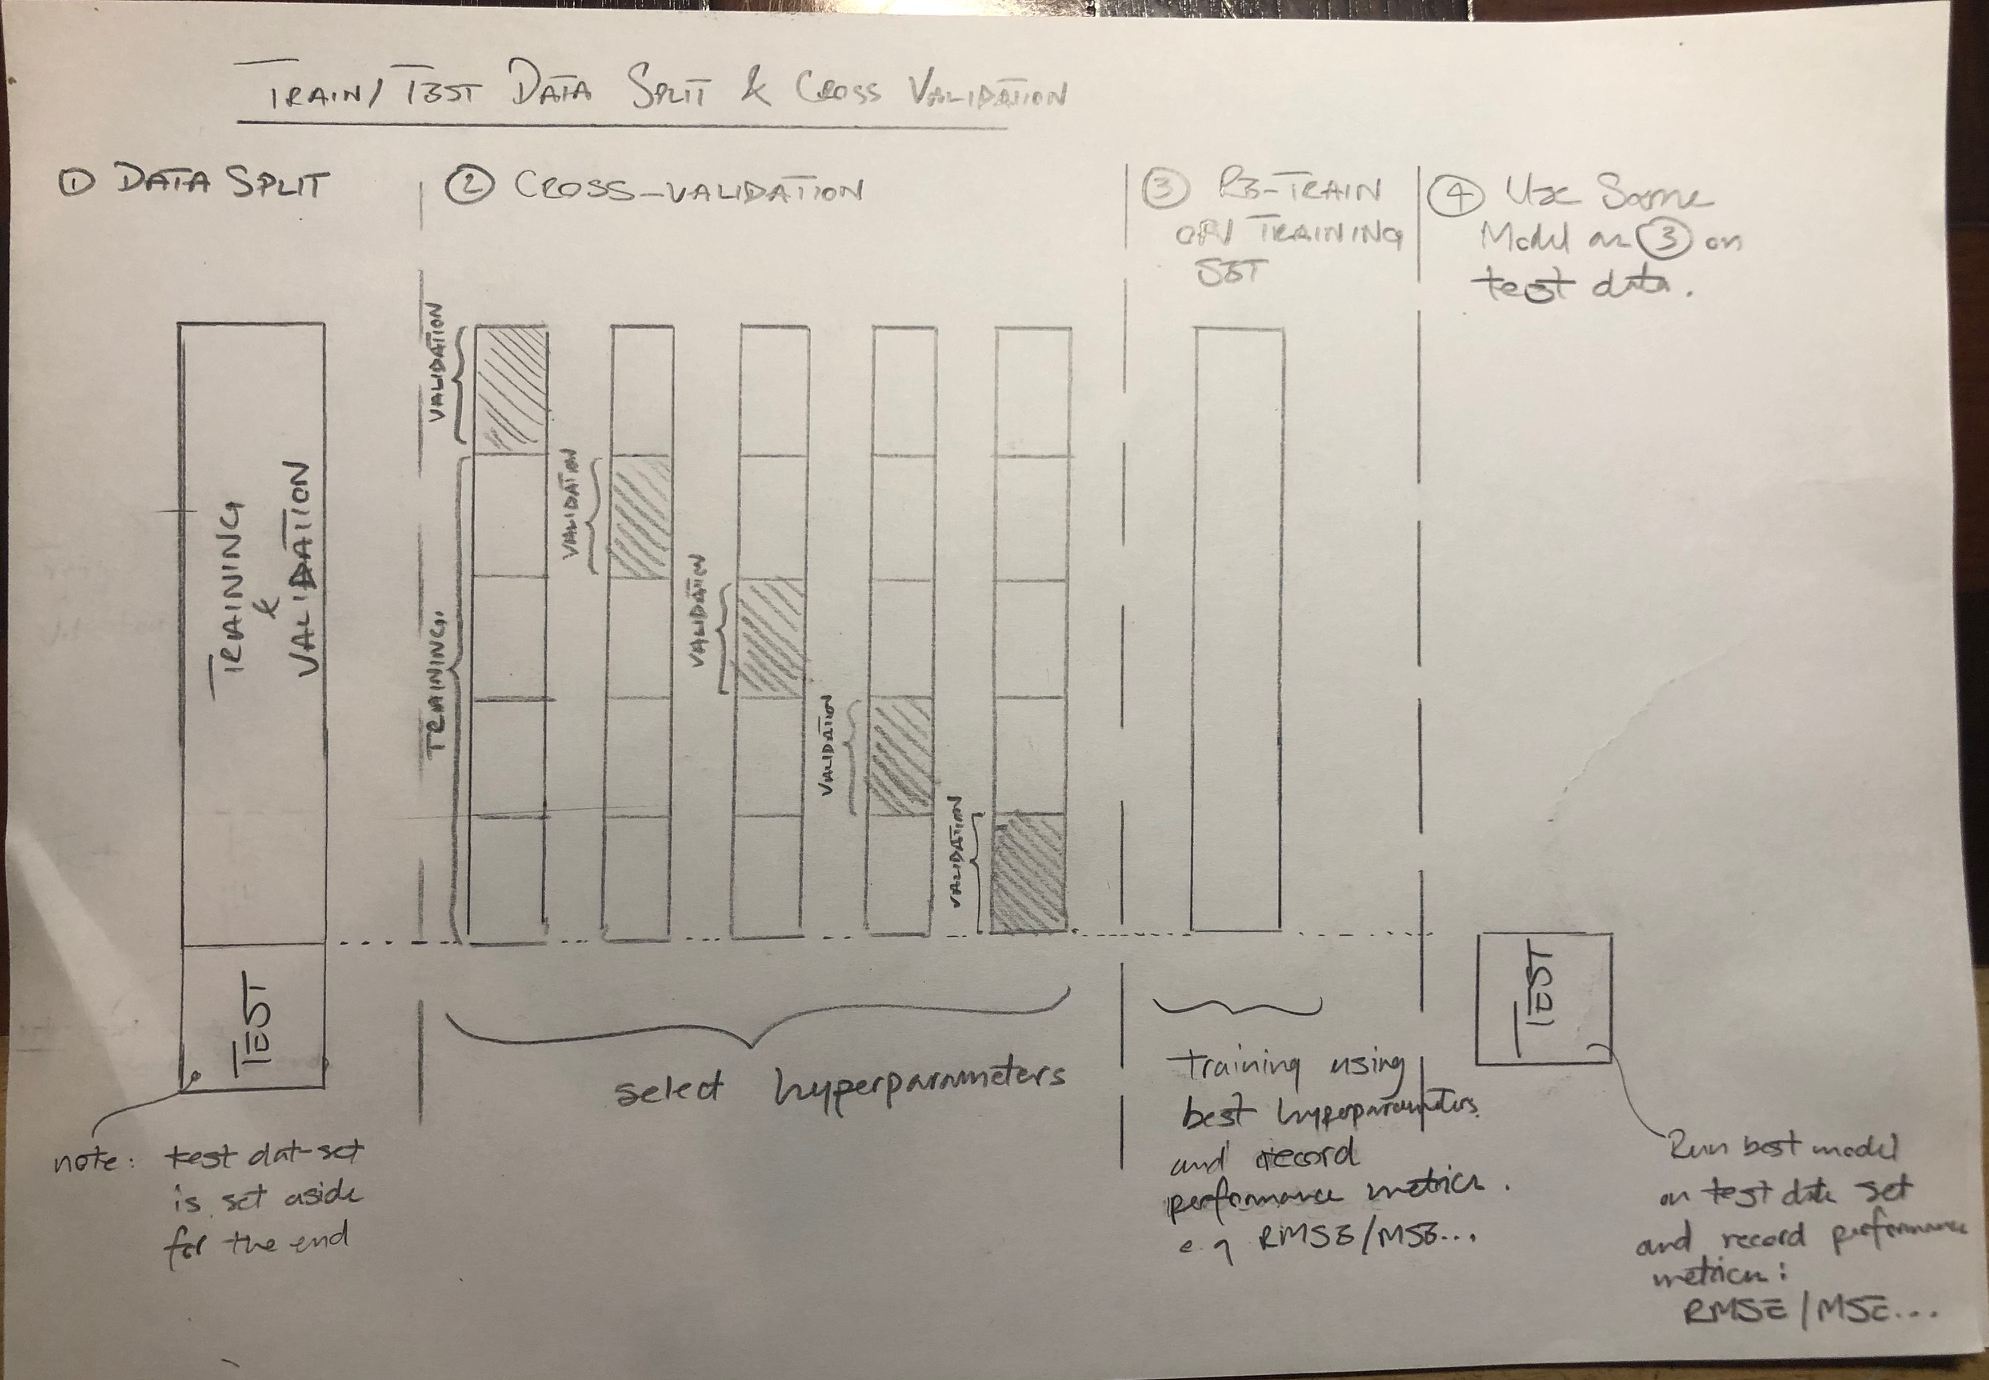
\includegraphics[width=0.9\linewidth]{./figures/Ch7fig0}
    \caption{Methodology used for model training, validating and testing}\label{Ch7Fig:1}
\end{figure}


The training process (steps 2 and 3 above) for the HMM model is slightly different.

For the selected hyperparameters, the HMM model is trained using maximum likelihood of the training data occurrence given the model. i.e. the HMM model found is the mostly likely model to have generated the training data. This model is then evaluated on the likelihood of the validation data and the process is repeated for the next k-fold. In contrast to the classical models where measures performance measures such as RMSE and Score are reported, HMM being a Bayesian model is evaluated using the likelihood criteria and a prediction is made based on a probability distribution.

\subsection{Data wrangling}


Data wrangling (also called data transformation or data munging) involves transforming the raw data into a suitable form for consumption by machine learning models.

The supervised (MLPRegressor, Ridge, BayesianRidge) and unsupervised (HMM) models we are investigating as part of this study require data to be in different shapes.

Supervised models expect data that contains both the input and the target, collectively referred to as labelled data. For this reason our chosen supervised models (Mlpregressor, Ridge, and BayesianRidge) need to be transformed into labelled data. The data is fitted into two matrices, a $X$ matrix (input data) and a $y$ matrix (labelled data), as shown in Figure~\ref{Ch7Fig:2}.

\begin{figure}[!ht]\centering
    \begin{tikzpicture}[x=100pt,y=100pt]
        \coordinate (X) at (-5pt,0);
        \coordinate (Y) at (0,-5pt);
        \coordinate (BL) at (0,0);
        \coordinate (TR) at (1,1);
        \coordinate (BR) at (BL-|TR);
        \coordinate (TL) at (BL|-TR);
        \coordinate (CL) at ($(BL)!0.5!(TL)$);
        \coordinate (CR) at ($(BR)!0.5!(TR)$);
        \coordinate (CT) at ($(TL)!0.5!(TR)$);
        \coordinate (bl) at (1.1,0);
        \coordinate (tr) at (1.3,1);
        \coordinate (br) at (bl-|tr);
        \coordinate (tl) at (bl|-tr);
        \coordinate (ct) at ($(tl)!0.5!(tr)$);

        \draw[thick,draw=black,fill=COL1] (BL) rectangle (TR);
        \draw[thick,draw=black,fill=COL1] (bl) rectangle (tr);

        \node[above] at (CT) {$X$};
        \node[above] at (ct) {$y$};

        \begin{scope}[>=latex,every node/.style={midway,font=\footnotesize}]
        \draw[<->] (CL) -- (CR)
            node[above] {fixed history}
            node[below] {e.g. 4 hours};

        \draw[<->] ([yshift=-5pt]BL) -- (Y-|BR) node[below] {Features};
        \draw[<->] (X|-BL)--(X|-TL) node[above,sloped] {Samples};

        \draw[<->] (Y-|bl)--(Y-|br) node[below] {Output=1};
        \end{scope}
    \end{tikzpicture}
    \caption{RFQ data transformed into an input matrix `$X$' and labelled column matrix utput `$y$' }\label{Ch7Fig:2}
\end{figure}

The rows in matrix `$X$' are a set by the number of samples in the dataset and the features equate to the history of RFQ's and `$y$' is a columnar target matrix of size (samples $\times$ 1), and it represents the RFQ counts for each bin. The $(X,y)$ matrix was produced 8 times, each instance corresponding to the data files in Table~\ref{Ch7Tab1}. As previously mentioned this study settled on investigating 15minute bin widths and the files in Tables [xx] are consistent with that. Files 1--4 represent labelled data for feature RFQ count, and files 5-8 represent features RFQ count and RFQ notionals. The 30, 1hr, 2hr and 4hr time variations refer to the length of history used in each file. For example a 30minute history is comprised of two 15minute columns for the $'X'$ input matrix.

\begin{table}[!ht]\centering\small
    \caption{Varying histories of labelled data used for supervised models}\label{Ch7Tab1}
    \begin{tabular}{cll}
        \toprule
        \bfseries\# & \bfseries Files & \bfseries Description\\
        \midrule
        1 & 30min.csv           & 30 minute RFQ count history              \\
        2 & 1hr.csv             & 1 hour RFQ count history                 \\
        3 & 2hr.csv             & 2 hour RFQ count history                 \\
        4 & 4hr.csv             & 4 hour RFQ count history                 \\
        5 & notional\_30min.csv & 30 minute RFQ count and notional history \\
        6 & notional\_1hr.csv   & 1 hour RFQ count and notional history    \\
        7 & notional\_2hr.csv   & 2 hour RFQ count and notional history    \\
        8 & notional\_4hr.csv   & 4 hour RFQ count and notional history    \\
        \bottomrule
    \end{tabular}
\end{table}


Unlike the supervised models there is no need to transform RFQs into labelled data for the HMM as it can deal with `un-labelled' sequences. However, it was necessary to ensure that the `visible' RFQ data was formulated in such a way so that it plausibly obeys the Markov assumption made by the HMM. Hence as explained later in the report \textcolor{red}{Section[xx]} a `differences' method was used for the HMM model. The additional feature called 'notional' was obtained by calculating the average FX option notional size in each 15 minute 'bin'. The average notionals were subsequently mapped using Appendix Table~\ref{AppTab:1} and used as a second feature in the construction of files containing notionals in Table~\ref{Ch7Tab1} \\

\subsection{Conclusion}

\textcolor{red}{TODO}